\documentclass[12pt]{article}
\usepackage{amsmath}
\usepackage{graphicx}
\usepackage{float}
\begin{document}
\title{Electrical Engineering 141, Homework 4}
\date{February 8th, 2019}
\author{Michael Wu\\UID: 404751542}
\maketitle

\section*{Problem 1}

\paragraph{a)}

From the Internal Model Principle, if \(\frac{s}{s+3}C(s)\) includes all the poles of \(R(s)\) as poles,
then the closed loop system can track a unit step reference input with zero steady state error. Since
\(R(s)=\frac{1}{s}\) has a pole at \(s=0\), we can design a compensator \(C(s)\) such that it tracks
the input with zero steady state error.

\paragraph{b)}

From the Internal Model Principle, we can set \(C(s)=\frac{1}{s^2}\) in order for the open loop transfer
function to contain a pole at \(s\).

\paragraph{c)}

We have the following transfer functions.
\begin{align*}
    Y(s)&=\frac{1}{s(s+3)}(R(s)-Y(s))\\
    \frac{Y(s)}{R(s)}&=\frac{1}{1+s(s+3)}\\
    H_{ry}(s)&=\frac{1}{s^2+3s+1}
\end{align*}
\begin{align*}
    Y(s)&=\frac{s}{s+3}\left(W(s)-\frac{1}{s^2}Y(s)\right)\\
    \frac{Y(s)}{W(s)}&=\frac{s^2}{1+s(s+3)}\\
    H_{wy}(s)&=\frac{s^2}{s^2+3s+1}
\end{align*}
\begin{align*}
    U(s)&=\frac{1}{s^2}\left(R(s)-\frac{s}{s+3}U(s)\right)\\
    \frac{U(s)}{R(s)}&=\frac{s+3}{s(1+s(s+3))}\\
    H_{ru}(s)&=\frac{s+3}{s(s^2+3s+1)}
\end{align*}
\begin{align*}
    U(s)&=-\frac{1}{s(s+3)}(W(s)+U(s))\\
    \frac{U(s)}{W(s)}&=-\frac{1}{s(s+3)+1}\\
    H_{wu}(s)&=-\frac{1}{s^2+3s+1}
\end{align*}
The transfer functions \(H_{ry}(s)\) and \(H_{wu}(s)\) are well behaved since they only have poles in the negative portion of the
\(s\) plane. The transfer function \(H_{wy}\) will also cause unit step disturbances to go to zero, so it is stable. However,
the transfer function \(H_{ru}(s)\) has \(s=0\) as a pole. So this means that \(u(t)\) will become unstable and grow without bound
when \(r(t)\) is the unit step function. So even though letting \(C(s)=\frac{1}{s^2}\) allows us to track the input with zero
steady state error, it causes our system to become unstable. Thus we cannot implement this compensator in real life.

\section*{Problem 2}

\paragraph{a)}

Since \(P(s)\) already contains \(s=0\) as a pole, the simplest compensator that ensures zero steady state error is \(C(s)=1\).
This can be verified by solving the following equation.
\begin{align*}
    Y(s)&=\frac{1}{s} + \frac{1}{s}\left(\frac{1}{s}-Y(s)\right)\\
    Y(s)&=\frac{1}{s+1}+\frac{1}{s(s+1)}\\
    Y(s)&=\frac{1}{s}
\end{align*}
So the output is indeed the unit step response.

\paragraph{b)}

If we use the compensator \(C(s)=1\), then our output is given by the following equation.
\begin{align*}
    Y(s)&=\frac{1}{s} + \frac{1}{s}\left(\frac{2}{s}-Y(s)\right)\\
    Y(s)&=\frac{1}{s+1}+\frac{2}{s(s+1)}\\
    Y(s)&=-\frac{1}{s+1}+\frac{2}{s}
\end{align*}
This has an output with a steady state of 2, so our previous compensator would not work.
We can instead choose a new compensator \(C(s)=2+\frac{1}{s}\). This ensures that
the system remains stable while also including the pole \(s=0\) of \(W(s)\) in the poles
of the compensator. The system remains stable because the sensitivity function
becomes the following.
\begin{align*}
    \frac{1}{1+P(s)C(s)}&=\frac{1}{1+\frac{1}{s}\left(2+\frac{1}{s}\right)}\\
    &=\frac{s^2}{s^2+2s+1}\\
    &=\frac{s^2}{(s+1)^2}
\end{align*}
This has two negative real poles, so it is stable. Furthermore, the gang of four becomes
the following.
\begin{align*}
    \frac{P(s)}{1+P(s)C(s)}&=\frac{s}{(s+1)^2}\\
    \frac{C(s)}{1+P(s)C(s)}&=\frac{2s^2+s}{(s+1)^2}\\
    \frac{P(s)C(s)}{1+P(s)C(s)}&=\frac{2s+1}{(s+1)^2}\\
\end{align*}
These are all stable, so our system is stable.

\paragraph{c)}

We can solve the following equation to obtain the answer.
\begin{align*}
    E(s)&=R(s)-(W_2(s)+P(s)(W_1(s)+C(s)E(s)))\\
    E(s)&=\frac{1}{s^2}-\left(\frac{1}{s}+\frac{1}{s}\left(\frac{1}{s}+\left(2+\frac{1}{s}\right)E(s)\right)\right)\\
    E(s)&=\frac{1}{s^2}-\frac{1}{s}-\frac{1}{s^2}-\left(\frac{2s+1}{s^2}\right)E(s)\\
    E(s)&=-\frac{s}{(s+1)^2}
\end{align*}
From the Final Value Theorem we can see that since \(\lim_{s\to0} sE(s)=0\), the steady state tracking
error will also be zero.

\paragraph{d)}

Our loop transfer function is the following.
\[P(s)C(s)=\frac{2s+1}{s^2}\]
Therefore our system is a type 2 system. The value of the corresponding error constant \(K_2\) is the following.
\[\lim_{s\to0} 2s+1 = 1\]

\paragraph{e)}

We can solve the following equation to obtain the answer.
\begin{align*}
    E(s)&=R(s)-(W_2(s)+P(s)(W_1(s)+C(s)E(s)))\\
    E(s)&=\frac{1}{s^2}-\left(\frac{1}{s^2}+\frac{1}{s}\left(\frac{1}{s}+\left(2+\frac{1}{s}\right)E(s)\right)\right)\\
    E(s)&=\frac{1}{s^2}-\frac{1}{s^2}-\frac{1}{s^2}-\left(\frac{2s+1}{s^2}\right)E(s)\\
    E(s)&=-\frac{1}{(s+1)^2}
\end{align*}
From the Final Value Theorem we can see that since \(\lim_{s\to0} sE(s)=0\), the steady state tracking
error will also be zero.

\paragraph{f)}

No we cannot achieve zero steady state tracking error with the same compensator as earlier. This is because the
compensator \(C(s)\) must include the unstable poles of \(W(s)\) as poles. If \(W(s)\) is the unit ramp function,
it will have two poles at \(s=0\) while our compensator \(C(s)=2+\frac{1}{s}\) only has one pole at \(s=0\).
We could modify our compensator to become \(C(s)=3+\frac{3}{s}+\frac{1}{s^2}\) in order to have two poles at
\(s=0\). This leads to a stable system because the sensitivity function becomes the following.
\begin{align*}
    \frac{1}{1+P(s)C(s)}&=\frac{1}{1+\frac{1}{s}\left(3+\frac{3}{s}+\frac{1}{s^2}\right)}\\
    &=\frac{s^3}{s^3+3s^2+3s+1}\\
    &=\frac{s^3}{(s+1)^3}
\end{align*}
The gang of four then becomes the following.
\begin{align*}
    \frac{P(s)}{1+P(s)C(s)}&=\frac{s^2}{(s+1)^3}\\
    \frac{C(s)}{1+P(s)C(s)}&=\frac{3s^3+3s^2+s}{(s+1)^3}\\
    \frac{P(s)C(s)}{1+P(s)C(s)}&=\frac{3s^2+3s+1}{(s+1)^3}\\
\end{align*}
Since there are no poles in the closed right half plane, our system is stable.

\paragraph{g)}

We have the following equations.
\begin{align*}
    Y(s)&=W_2(s)+P(s)C(s)(R(s)-Y(s))\\
    Y(s)&=\frac{W_2(s)+P(s)C(s)R(s)}{1+P(s)C(s)}\\
    R(s)&=\frac{1}{s}+\frac{1}{s^2+1}\\
    W_2(s)&=\frac{s}{s^2+\frac{1}{10000}}
\end{align*}
Then plugging in yields the following expression.
\[Y(s)=\frac{10000s^2(s+1)}{(s^2+s+1)(10000s^2+1)} + \frac{1}{s(s^2+1)}\]
Notice that the right term has poles \(s=\pm j\), therefore this output signal does
not have a steady state value. It will oscillate around the value 1.

\section*{Problem 3}

\paragraph{a)}

We have the following.
\begin{align*}
    Y(s)&=H(s)(R(s)-F(s)Y(s))\\
    \frac{Y(s)}{R(s)}&=\frac{H(s)}{1+H(s)F(s)}
\end{align*}

\paragraph{b)}

\begin{align*}
    S_H^{H_{cl}}&=\frac{\frac{dH_{cl}}{H_{cl}}}{\frac{dH}{H}}\\
    &=\frac{dH_{cl}}{dH}\frac{H}{H_{cl}}\\
    &=\frac{1}{(1+H(s)F(s))^2}(1+H(s)F(s))\\
    &=\frac{1}{1+L(s)}
\end{align*}

\paragraph{c)}

\begin{align*}
    S_F^{H_{cl}}&=\frac{\frac{dH_{cl}}{H_{cl}}}{\frac{dF}{F}}\\
    &=\frac{dH_{cl}}{dF}\frac{F}{H_{cl}}\\
    &=-\frac{H(s)^2}{(1+H(s)F(s))^2}\frac{F(s)(1+H(s)F(s))}{H(s)}\\
    &=-\frac{H(s)F(s)}{1+H(s)F(s)}\\
    &=-\frac{L(s)}{1+L(s)}
\end{align*}

\paragraph{d)}

The two results are related since \(S_H^{H_{cl}}-S_F^{H_{cl}}=1\).
We would want \(|L(s)|>>1\) in order to reduce the closed-loop sensitivity
to variations in the feedforward element. We would want \(|L(s)|\approx 0\)
in order to reduce the closed-loop sensitivity to variations in the feedback
element. Based on these results, if we were designing a feedback amplifier
we would want our more accurate components in the feedback element. This
is because we don't want \(L(s)\) to be very small, since this would mean
that our feedback loop has little effect. If \(L(s)=0\), we might as well
not have a feedback loop at all. So then we should assume that \(L(s)\) is
very large and the feedforward element can handle large disturbances. So the
feedback element should contain the accurate components since it has the most
control over the output of the loop.

\section*{Problem 4}

\paragraph{a)}

If \(H>>1\) then we can approximate our closed loop transfer function as \(\frac{1}{F(s)}\).

\paragraph{b)}

Let the open loop gain be denoted by \(G(t)=\frac{Hf(y(t))}{y(t)}\). Then we have the following.
\begin{align*}
    y(t)&=H(r(t)-f(y(t)))\\
    y(t)+Hf(y(t))&=Hr(t)\\
    (1+G(t))y(t)&=Hr(t)\\
    \frac{y(t)}{r(t)}&=\frac{H}{1+G}
\end{align*}
If the value \(H\) is very large, then this result becomes the following.
\begin{align*}
    \frac{y(t)}{r(t)}&=\frac{y(t)}{f(y(t))}\\
    f(y(t))&=r(t)\\
    y(t)&=f^{-1}(r(t))
\end{align*}
Thus for \(H>>1\), our closed-loop system acts like the inverse of the feedback element.

\paragraph{c)}

Since we assume an ideal OpAmp, all the current through the resistor also goes
through the diode. We also assume that the voltage at the negative terminal of the OpAmp
is negligible, so we can treat it as zero. Then we have the following.
\begin{align*}
    V_\text{in}&=IR\\
    V_\text{in}&=I_sRe^{-\frac{V_\text{out}}{V_T}}\\
    -\frac{V_\text{out}}{V_T}&=\ln\left(\frac{V_\text{in}}{I_sR}\right)\\
    V_\text{out}&=-V_T\ln\left(\frac{V_\text{in}}{I_sR}\right)
\end{align*}

\section*{Problem 5}

\paragraph{a)}

The loop transfer function is the following.
\[L(s)=P(s)C(s)=\frac{3140(s+10)}{s^2(s+100)}\]

\paragraph{b)}

The sensitivity function is the following.
\[S(s)=\frac{1}{1+L(s)}=\frac{s^2(s+100)}{s^2(s+100)+3140(s+10)}\]

\paragraph{c)}

I ran the following code.
\begin{verbatim}
s = tf('s');
S = s^2*(s + 100)/(s^2*(s + 100) + 3140*(s + 10));
set(gcf,'color','w');
bodemag(S);
export_fig problem5c.pdf;
[Gm, Pm, Wcg, Wcp] = margin(S);
\end{verbatim}
This generated the following plot.
\begin{figure}[H]
    \begin{center}
        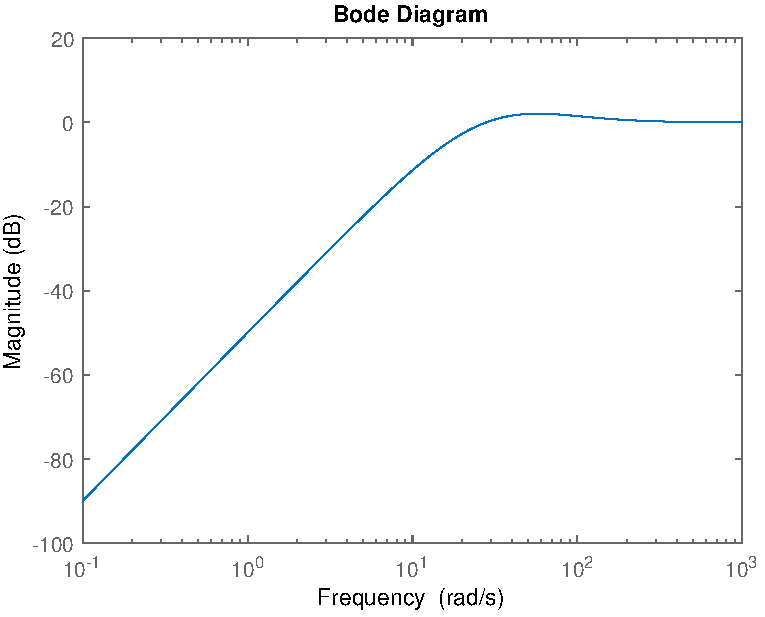
\includegraphics[width=3.5in]{problem5c.pdf}
    \end{center}
\end{figure}
I also obtained a crossover frequency of \(27.8076\) rad/s.

\paragraph{d)}

Disturbances with a frequency below \(27.8076\) rad/s would be attenuated.

\paragraph{e)}

The closed loop transfer function is the following.
\[T(s)=\frac{L(s)}{1+L(s)}=\frac{3140(s+10)}{s^2(s+100)+3140(s+10)}\]
This has poles at \(-48.98\), \(-28.61\), and \(-22.40\). It has one
zero at \(-10\). This system is stable since all its poles lie in the
open left half plane.

\paragraph{f)}

The step response is shown below.
\begin{figure}[H]
    \begin{center}
        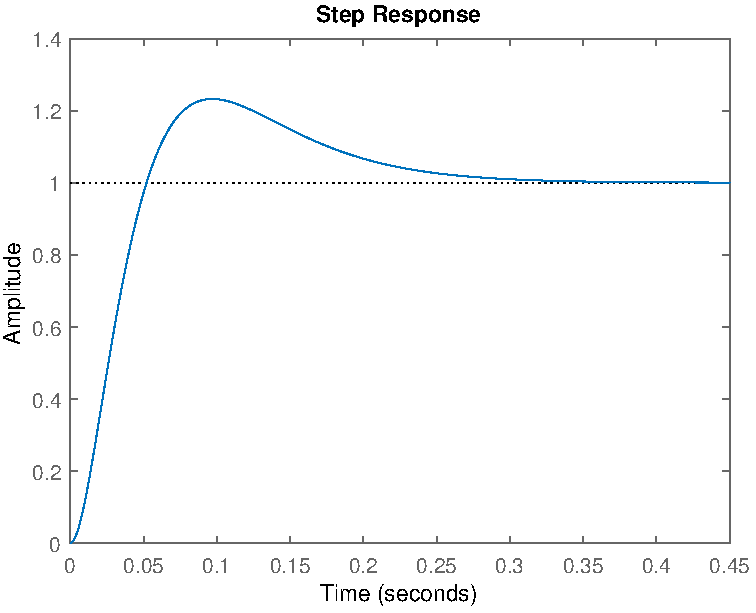
\includegraphics[width=3.5in]{problem5f.pdf}
    \end{center}
\end{figure}

\paragraph{g)}

\[\delta_p(s)=\frac{12.56}{s^2+0.707s+28}\frac{s^2}{6.28}=\frac{2s^2}{s^2+0.707s+28}\]

\paragraph{h)}

Our new loop transfer function is the following.
\begin{align*}
    L(s)&=\frac{3140(s+10)}{s^2(s+100)}+\frac{6280(s+10)}{(s+100)(s^2+0.707s+28)}\\
    &=\frac{3140(s+10)(s^2+0.707s+28)+6280s^2(s+10)}{s^2(s+100)(s^2+0.707s+28)}
\end{align*}
Then our closed loop transfer function is the following.
\[T(s)=9420\frac{s^3+10.2357s^2+11.69s+93.3333}{s^5+100.707s^4+9518.7s^3+99220s^2+110120s+879200}\]
This has poles at the following locations.
\[s=-44.57 \pm 80.56j,-11.33,-0.12 \pm 3.02j\]
So this system is stable since all of its poles lie in the open left half plane.

\paragraph{i)}

The bode plot is shown below.
\begin{figure}[H]
    \begin{center}
        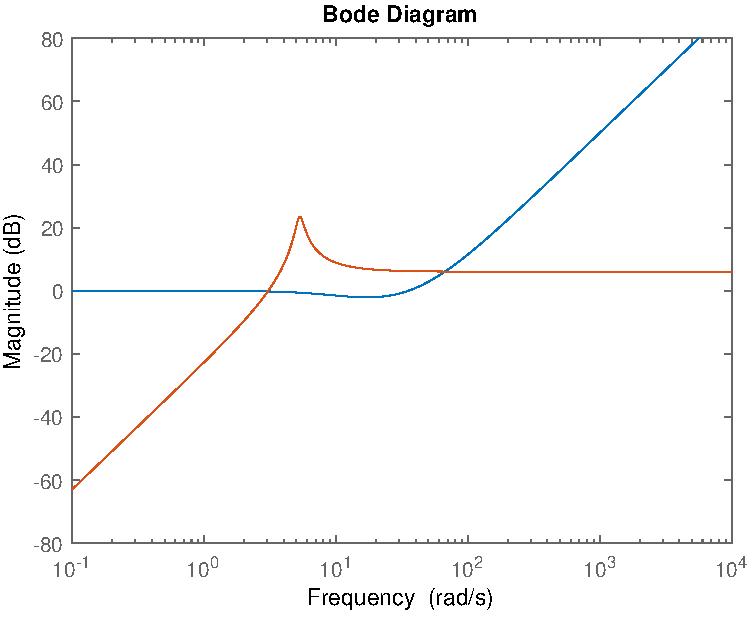
\includegraphics[width=3.5in]{problem5i.pdf}
    \end{center}
\end{figure}
The line that is mostly flat then begins increasing on the right is \(\frac{1}{|T(j\omega)|}\)
and the line that is increasing on the left then goes to zero is \(|\delta_P(j\omega)|\).
This does not satisfy the Robust Stability criteria because the multiplicative plant
perturbation has a greater magnitude than the inverse of the closed loop transfer function
for some frequencies. At these frequencies our system would not be stable.

\paragraph{j)}

The loop transfer function is the following.
\[L(s)=C_1(s)P(s)=\frac{6.28\times0.0005(s+0.01)}{s^2(s+0.1)}\]
The closed loop transfer function is the following.
\[T_1(s)=\frac{L(s)}{1+L(s)}=\frac{0.00314s+0.0000314}{s^3+0.1s^2+0.00314s+0.0000314}\]
This has poles at the following locations.
\[s=-0.049, -0.029, -0.022\]
So this system is stable since all its poles lie in the open left half plane.

\paragraph{k)}

The bode plot is shown below.
\begin{figure}[H]
    \begin{center}
        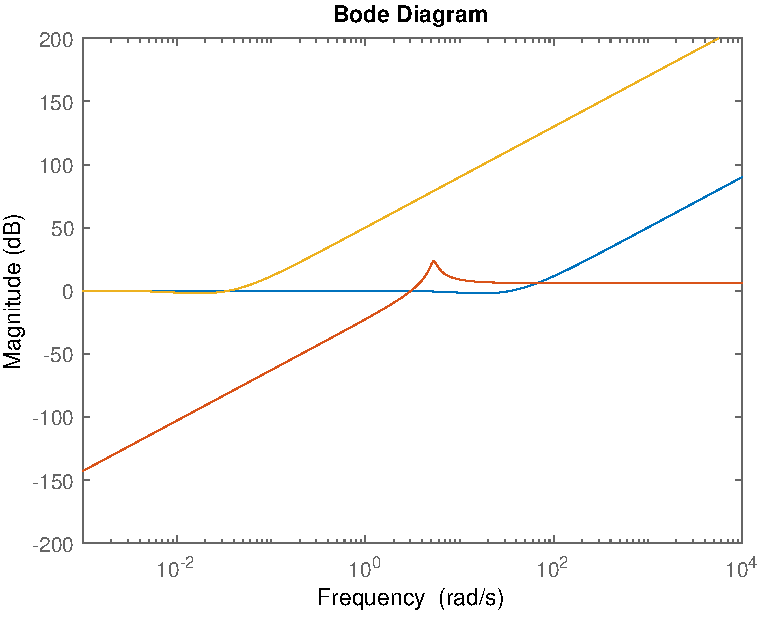
\includegraphics[width=3.5in]{problem5k.pdf}
    \end{center}
\end{figure}
The new line that begins to rise on the left is \(\frac{1}{|T_1(s)|}\). This does
satisfy the Robust Stability criteria because the multiplicative plant perturbation
has a smaller magnitude than the inverse of the closed loop transfer function for all
frequencies.

\paragraph{l)}

The step response is shown below.
\begin{figure}[H]
    \begin{center}
        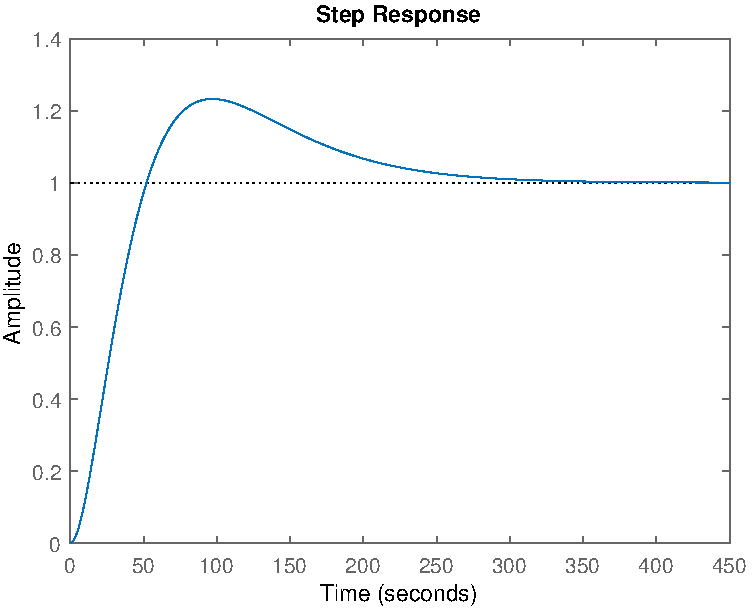
\includegraphics[width=3.5in]{problem5l.pdf}
    \end{center}
\end{figure}
The time scale in this diagram is much longer than with the previous compensator. This
illustrates the trade off between robustness and stability, as our robust system does
not cancel out disturbances very quickly.

\paragraph{m)}

The closed loop transfer function is the following.
\[T(s)=\frac{0.00942s^3+0.0022294s^2+0.0879222s+0.00008792}{s^5+0.807s^4+28.0801s^3+2.80223s^2+0.0879222s+0.00008792}\]
This has zeros at the following points.
\[s=-0.35 \pm 5.28j,-0.049 \pm 0.024j,-0.001\]

\end{document}